\subsection{Optimization vs. Learning}

The goal of optimization in \ac{dl} is to maximize the performance on some measure P. Since P might be intractable (0/1 accuracy not differentiable), we introduce a surrogate loss function \pL, which is \b{tractable, differentiable} and \b{might enable better generalization}.\\
In practice, optimizing \f{\mathcal{L}} directly may not generalize well (overfitting). In order to mitigate this, we can add regularization terms to the loss function.

\definition{\b{Learning} in contrast is distinguished from pure optimization by the following points:
\begin{itemize}
    \item May have to use surrogate instead of the real objective such as softmax instead of hard-max.
    \item Optimization on partial data distribution instead of the real distribution.
    \item Often introduces regularization term to generalize.
    \item Requires the summation over given data points, so computationally expensive for a large dataset.
\end{itemize} }

\subsection{Gradient-Based Optimization}
In order to minimize the loss of the model, we need to find a global minimum of \pL. Even though this could be solved analytically (the gradient is \f{0} at a minimum), this is not feasible in practice. Instead, we use the numerical (iterative) method of \b{Gradient Descent}.\\
The algorithm is described in the following figure:
\vspace{0.3cm}
\begin{figure}[h]
    \centering
    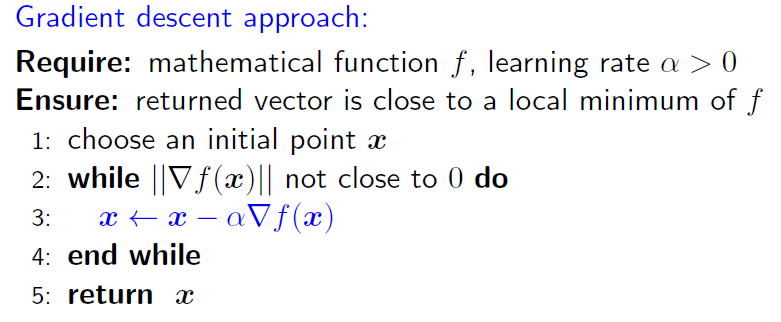
\includegraphics[width=0.6\textwidth]{gd.png}
\end{figure}

\subsection{Ill-Conditioning}
The condition number \f{\kappa(Q)} of a matrix \f{Q} with eigenvalues \f{\lambda} is defined as \f{\kappa(Q)=\frac{\lambda_{\max}}{\lambda_{\min}}}.\\
Matrices with large condition number are called \b{ill-conditioned}.\\
Ill-conditioned matrices drastically hurt convergence performance by causing \b{zig-zag behavior} (one dimension contributes more than the others)!\\[0.5em]

There are two methods to mitigate this issue in practice: \b{momentum} and \b{preconditioning}.

\definition{\b{Momentum} takes into account the direction of the previous gradients by adding an extrapolation step (\f{\beta}) to the gradient step:
\cf{
    x_{k+1}=x_k - \alpha\nabla f(x_k) + \beta(x_k - x_{k-1}) = x_k - \alpha\sum_{i=0}^{k}\beta^{k-i}g_i
}}

\definition{\b{Preconditioning} makes use of a \b{preconditioning matrix} \f{D_k} (positiv definite and symmetric) to pre-multiply the gradients by \f{D_k} in order to scale the gradients:
\cf{
    x_{k+1} = x_k - \alpha D_k \nabla f(x_k)
}
\b{Note:} The best scaling is the inverse of the Hessian matrix \f{D_k = \nabla^2f(x_k)^{-1}} (Newton's method). The problem with Newton's method is that it is also attracted to maximizers.}

\subsection{Challenges of Optimization}
\begin{itemize}
    \item \b{Non-Convexity:} The model m is a highly non-convex function (saddle points very likely).
    \item \b{Large datasets:} In modern datasets, \f{N} is large (makes gradient calculation very expensive).
    \item \b{High dimensionality:} In modern neural networks, \f{d} is very large.
    \item \b{Structure of the network:} Can yield hard-to-optimize response surfaces.
\end{itemize}
Furthermore, the following properties in the structure of neural networks make optimizations harder:
\begin{enumerate}
    \item \b{Cliff-like surfaces in the searching space:} he gradients suddenly drop or rise signifcantly at some points, especially in \acp{rnn}.
    \item \b{Gradient vanishing and exploding:} Since we have to multiply matrices again and again, each value is going to be very small or large by the power factor.
\end{enumerate}

\subsection{\ac{sgd}}
While standard gradient descent handles learning by epoch, SGD computes the loss value using only a part of the dataset. Note that learning by epoch is to learn all the training data at the same time. Typically, the optimization by gradient descent is stable, but it takes a lot more time. Therefore, we use so-called \b{mini-batches}, i.e. a part of the dataset, for one update step. SGD stochastically picks a batch of data points and learns the batch at each step.\\
SGD is preferred due to the following reasons:

\begin{enumerate}
    \item Much quicker training allows much more iterations.
    \item Since the standard error of empirical loss function against true loss function decreases by the order of \f{O(\frac{1}{\sqrt{B}})} where \f{B} is the batch size, a larger batch size does not make a big difference.
    \item The training dataset can include many similar data points, so mini-batch learning is likely to yield similar results to that of full-set training.
    \item Since mini-batch includes less data points and the standard error is larger, the neural networks are not likely to overfit the statistics of the given data distribution.
\end{enumerate}

\b{Note:} We typically want to set the batch size as large as possible given memory constraints. However, small batch sizes can have a regularizing effect (small batch size requires lower learning rates). In order to mitigate biases of the data collection process, we randomly shuffle the training data before drawing batches.

\subsection{Learning Rate Schedules}
Setting the learning rate \f{\alpha} correctly is very important for good model convergence. Too low a learning rate can drastically slow down convergence, while too high a learning rate might lead to divergence.\\[0.5em]
Generally, using a fixed learning rate is not a good practice, as SGD would never converge. For this reason, dynamic learning rate scheduling is used:
\begin{itemize}
    \item \b{Linear decay:} Until iteration \f{\tau}: \f{\alpha_k = (1-b)\alpha_0 + b\alpha_\tau,} with \f{b=k/\tau}. Then constant.
    \item \b{Exponential decay:} \f{\alpha_k = b\alpha_{k-1}=b^k\alpha_0}
    \item \b{Step decay:} Decay by a factor (e.g. 10) every n steps.
    \item \b{Cosine decay:} \f{\alpha_k = \frac{1}{2}(1+\cos(\frac{k}{n}\pi))\times \alpha_0}, with \f{n} being the total number of epochs.
    \item \b{SGD with warm restarts (SGDR):} Consists of multiple repeated steps
    \begin{enumerate}
        \item Quickly cool down \f{\alpha} to zero
        \item Heat up \f{\alpha} again
        \item Cool down \f{\alpha} more slowly.
    \end{enumerate}
\end{itemize}

\subsection{SGD with Momentum}
As introduced before, momentum \f{v} (velocity) is an exponentially moving average of past gradients. This makes updates smoother by keeping a history. Update step:
\cf{v \leftarrow \beta v - \alpha \hat{g}}
\cf{\theta \leftarrow \theta + v}
Advantages of using momentum are:
\begin{itemize}
    \item Smoothes zig-zagging
    \item Accelerates learning at flat spots
    \item Slows down when signs of partial derivatives change
\end{itemize}
\b{Disadvantages}: additional parameter \f{\beta}, strong momentum might cause more zig-zagging

\subsection{Adaptive Gradient Algorithms}
The learning rate has to be adapted for convergence. However, to do so may require different learning rates for different dimensions. This is where adaptive gradient algorithms come into play:
\begin{enumerate}
    \item \b{AdaGrad:} Update step:
    \begin{enumerate}
        \item \f{r \leftarrow r + \hat{g} \odot \hat{g}\quad} (accumulate squared gradient)
        \item \f{\Delta\theta \leftarrow - \frac{\alpha}{\epsilon + \sqrt{r}} \odot \hat{g}\quad} (scale \f{\alpha} by root of cumulative squared gradient, \f{\epsilon << 1})
        \item \f{\theta \leftarrow \theta + \Delta\theta\quad} (update model weights)
    \end{enumerate}
    \begin{itemize}
        \item High learning rate for dimensions with small gradient.
        \item Sometimes decreases learning rate too early due to long influences of past gradients.
    \end{itemize}
    \item \b{RMSProp:} Update step:
    \begin{enumerate}
        \item \f{r \leftarrow \rho r + (1-\rho)\hat{g} \odot \hat{g}\quad} (EMA of squared gradient)
        \item \f{\Delta\theta \leftarrow - \frac{\alpha}{\epsilon + \sqrt{r}} \odot \hat{g}\quad}
        \item \f{\theta \leftarrow \theta + \Delta\theta\quad}
    \end{enumerate}
    \begin{itemize}
        \item \f{\rho} is a new hyperparameter controlling how quickly past gradients are forgotten.
    \end{itemize}
    \item \b{Adam:} Update step:
    \begin{enumerate}
        \item \f{t \leftarrow t + 1}
        \item \f{s \leftarrow \rho_1s + (1-\rho_1)\hat{g}\quad} (EMA of gradient)
        \item \f{r \leftarrow \rho_2r + (1-\rho_2)\hat{g} \odot \hat{g}\quad} (EMA of squared gradient)
        \item \f{\hat{s} \leftarrow \frac{s}{1-\rho_1^t}\quad} (correct bias in moving gradient estimate)
        \item \f{\hat{r} \leftarrow \frac{r}{1-\rho_2^t}\quad} (correct bias in sq. moving bias estimate)
        \item \f{\Delta\theta \leftarrow - \frac{\alpha}{\epsilon + \sqrt{\hat{r}}} \odot \hat{s}\quad}
        \item \f{\theta \leftarrow \theta + \Delta\theta\quad}
    \end{enumerate}
    \begin{itemize}
        \item \f{\rho_i} are decay rates for first and second moment.
        \item Extension of RMSProp with momentum and bias correction.
    \end{itemize}
\end{enumerate}